\subsection{Particle Clustering}

Once the semantic segmentation is done, their results get passed onto the spice GNN.
The purpose of this GNN is to group different voxels together if they belong to the same shower or track.
The SPICE (Sparsity-preserving Invariant Convolutional Embedding) model is a novel approach designed to address challenges in graph-based learning by leveraging sparsity and invariance principles.
At its core, SPICE utilizes convolutional operations that preserve the structural sparsity of graphs, which is crucial for efficiently processing large-scale and complex graph data.
Lucky for us, neutrino events are incredibly sparse.
By maintaining sparsity, SPICE reduces computational overhead and memory usage, making it scalable to larger graphs.
The invariant convolutional embeddings produced by SPICE ensure that the model is robust to transformations and perturbations in graph structures, such as node and edge additions or deletions, thereby enhancing its generalization capabilities.

In practical terms, SPICE integrates several advanced techniques to optimize graph learning tasks.
The model incorporates a sparse convolutional layer that operates directly on the non-zero elements of graph adjacency matrices, bypassing the need for dense matrix operations that can be computationally expensive.
Additionally, SPICE applies invariant transformations that allow the network to remain effective even when the graph undergoes structural changes.

\begin{figure}[H]
  % 
  \centering
  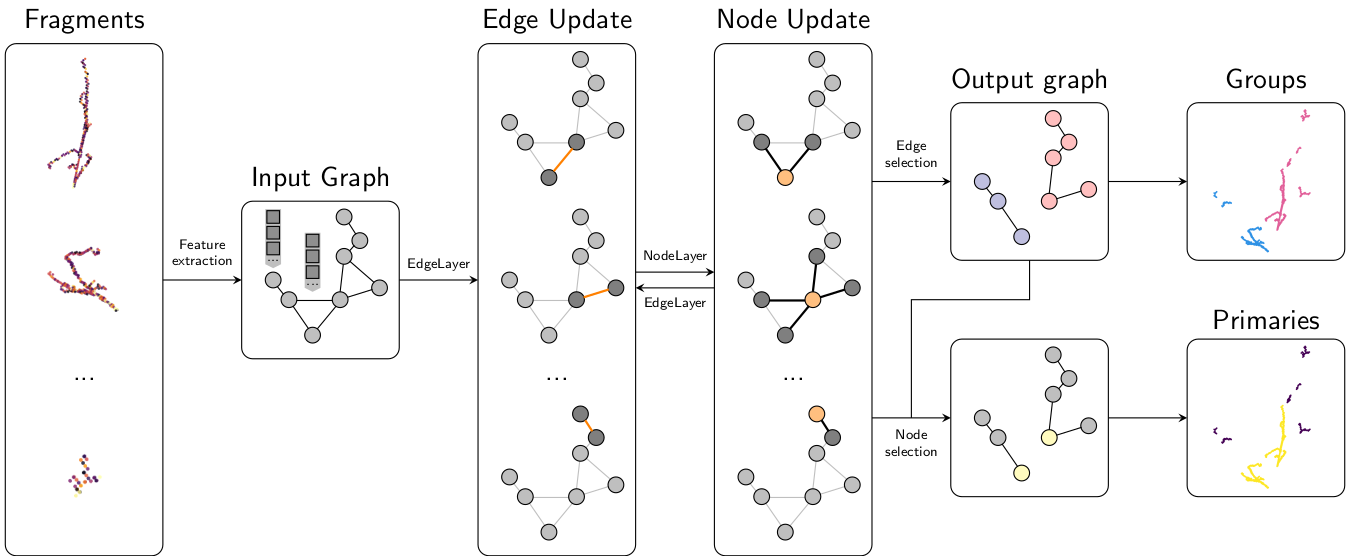
\includegraphics[width=120mm]{figures/gnn.png}
  \caption{Architecture of the clustering GNN}
  \label{gnn}
\end{figure}

This clustering is done in separate parts between the tracks and showers before coming together to cluster interactions.

\begin{figure}[H]
  % OWN
  \centering
  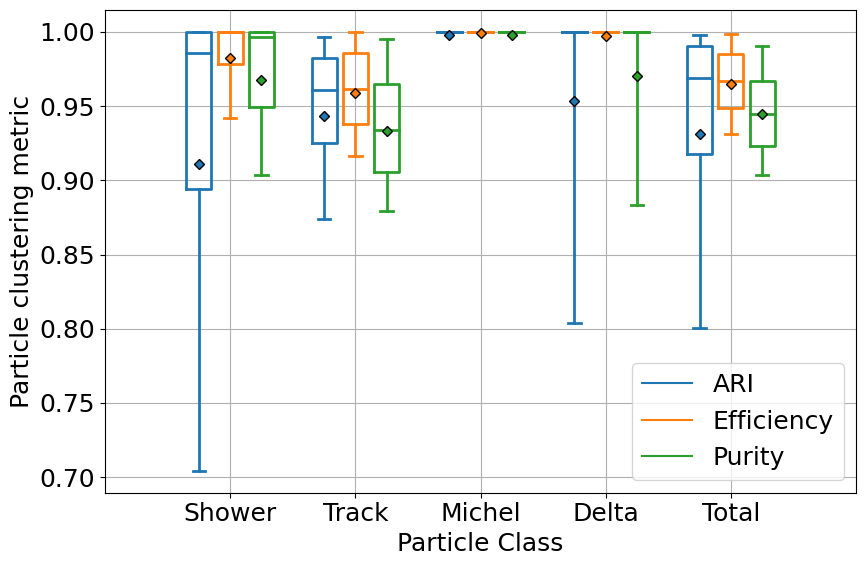
\includegraphics[width=120mm]{figures/clusteringPerformance.png}
  \caption{Box and whisker plot showing performance of clustering}
  \label{clusteringPerformance}
\end{figure}

\begin{itemize}
\item Efficiency: The proportion of true neutrino events correctly captured in their respective clusters, reflecting the model's ability to retain genuine signals.

\item Purity: The degree to which clusters consist of events from a single true category, minimizing cross-contamination from unrelated interactions.

\item ARI (Adjusted Rand Index): A metric comparing predicted and true clusters, adjusted for randomness, where higher values indicate better alignment in grouping neutrino events.
\end{itemize}

The graph shows that shower and track clustering performance is good.
The values of the Michel electrons are a bit misleading since there weren't any in the dataset being tested which is why it looks perfect.
It is not perfect and further development needs to be done on this.
  
Due to the modular nature of the $2 \times 2$ prototype , there can be quite large gaps between 2 parts of the same track or in the middle of a shower where the modules  switch over making the job of clustering more difficult than it would be in a monolithic detector.

